\documentclass{book}
\usepackage[top=20mm,bottom=20mm,left=20mm,right=20mm,a4paper]{geometry}
\usepackage{microtype,soul,filecontents}
\usepackage{pgf}
\usepackage{lettrine,caption,multicol}
\usepackage{xcolor}
\usepackage{lipsum,soul}
\usepackage{palatino}
\usepackage{calligra}
\usepackage[T1]{fontenc}
%\usepackage[spanish]{minitoc}
\usepackage{minitoc}
\usepackage{titlesec}
\usepackage{titletoc}
\setcounter{minitocdepth}{2}
\setlength{\mtcindent}{24pt}
\renewcommand{\mtcfont}{\small\rm}
\renewcommand{\mtcSfont}{\small\bf}
\renewcommand{\ptctitle}{Contenido}

\makeatletter
\usepackage[listings,theorems]{tcolorbox}
%\usepackage[charter]{mathdesign}
% \def\rmdefault{bch} % not scaled
% \def\ttdefault{blg}
\usepackage{xcolor,filecontents,ragged2e}
\definecolor{theblue} {rgb}{0.02,0.04,0.48}
\definecolor{thered}  {rgb}{0.65,0.04,0.07}
\definecolor{thegreen}{rgb}{0.06,0.44,0.08}
\definecolor{thegrey} {gray}{0.5}
\definecolor{theshade}{gray}{0.94}
\definecolor{theframe}{gray}{0.75}
\def\chaptername{Cap\' itulo}
\def\indexname{\' Indice}
\def\bibname{Bibliograf\'ia}
\def\contentsname{Contenido}
\newcommand\lorem{Fusce adipiscing justo nec ante. Nullam in enim.
 Pellentesque felis orci, sagittis ac, malesuada et, facilisis in,
 ligula. Nunc non magna sit amet mi aliquam dictum. In mi. Curabitur
 sollicitudin justo sed quam et quadd. \par}

\lstloadlanguages{[LaTeX]TeX, [primitive]TeX}

% Emphasis
\newcommand\emphasis[2][thered]{\lstset{emph={newcommand,def,gdef,#2},
   emphstyle={\ttfamily\textcolor{#1}}}}%

\lstset{language={[LaTeX]TeX},
      escapeinside={{(*@}{@*)}}, 
       numbers=left, gobble=0,
       stepnumber=1,numbersep=5pt, 
       numberstyle={\footnotesize\color{gray}},firstnumber=last,
       breaklines=true,
       framesep=5pt,
       basicstyle=\small\ttfamily,
       showstringspaces=false,
     % keywordstyle=\ttfamily\textcolor{thegreen},
      stringstyle=\color{orange},
      commentstyle=\color{black},
      rulecolor=\color{theshade},
      breakatwhitespace=true,
     showspaces=false,  % shows spacing symbol
      xleftmargin=0pt,
      xrightmargin=5pt,
      aboveskip=3pt plus1pt minus1pt, % compact the code looks ugly in type
      belowskip=7pt plus1pt minus1pt,  % user responsible to insert any skips
      backgroundcolor=\color{theshade}
}

\begin{filecontents*}{chapterx.sty}
\ProvidesPackage{chapters}[2012/04/07 v0.1 Typesetting chapters]
\newcommand\HUGE{\@setfontsize\Huge{38}{47}}
\newcommand\HHUGE{\@setfontsize\HHUGE{58}{67}}


\newenvironment{summary}
               {\list{}{\listparindent0pt %
                        \itemindent\listparindent
                        \leftmargin0pt
                        \rightmargin\leftmargin
                        \parsep\z@ \@plus\p@}%
                \item\relax\itshape}
               {\endlist}

% helper macros
\gdef\thinrule{\rule{\textwidth}{0.4pt}}
\gdef\mediumrule{\rule{\textwidth}{0.8pt}}
%% broad positions
\newif\if@left
\newif\if@right
\newif\if@center
\@leftfalse
\@rightfalse
\@centerfalse
% newifs for number position
\newif\if@lefttitle
\newif\if@righttitle
\newif\if@leftname
\newif\if@rightname
\newif\if@chapterspaceout\@chapterspaceoutfalse
\newif\if@titlespaceout\@chapterspaceoutfalse

%\section{Libraries} 

\def\cx@optionlist{}


\def\cx@optionlist{}

\def\cxuselibrary#1{\cxset{library/.cd,#1}}
%
% The library is added by inputting the file and setting the path accordingly.
\def\cx@add@library#1#2{%
  \cxset{library/#1/.code={\@ifundefined{cxlibrary@#1@loaded}{\input #2}{}}}%
  \DeclareOption{#1}{\edef\cx@optionlist{\cx@optionlist,#1}}%
}

\def\thickrule{\leavevmode \leaders \hrule height 3pt \hfill \kern \z@}


% Define a family for chapter styling keys
\pgfkeys{/chapter/.is family}



\def\cxset{\pgfqkeys{/chapter}} %Notice this is pgf q keys
% spent half the evening to debug it;)Aarg!!!
% We define keys for all major components
\cxset{%
  name/.code={\gdef\chaptername{#1}},
  color/.store in=\color@cx,
  color/.default=black,
  chapter font-family/.store in=\chapterfontfamily@cx,
  chapter font-weight/.store in=\chapterfontweight@cx,
  chapter font-size/.store in=\chapterfontsize@cx,
  chapter color/.store in=\chaptercolor@cx,
  chapter before/.store in=\chapterbefore@cx,
  chapter after/.store in=\chapterafter@cx,
  chapter spaceout/.is choice,
  chapter spaceout/soul/.code={\@chapterspaceouttrue},
  chapter spaceout/none/.code={\@chapterspaceoutfalse},
  % title keys
  title font-family/.store in=\titlefontfamily@cx,
  title font-family/.default=\rmfamily,
  title font-weight/.store in=\titlefontweight@cx,
  title font-size/.store in=\titlefontsize@cx,
  title font-color/.store in=\titlefontcolor@cx,
  title spaceout/.is choice,
  title spaceout/soul/.code={\@titlespaceouttrue},
  title spaceout/none/.code={\@titlespaceoutfalse},
  title font/.style={title font-family=#1},
  title before/.store in=\titlebefore@cx,
  title after/.store in=\titleafter@cx,
  title beforeskip/.store in=\titlebeforeskip@cx,
  title afterskip/.store in=\titleafterskip@cx,
  position/.is choice,
  position/left/.code={\@lefttrue},
  position/right/.code={\@righttrue},
  position/center/.code={\@centertrue},
% numbering options that are required
  numbering/.is choice,
% better to rename thechapter?
  numbering/roman/.code={\gdef\thechapter{\@roman\c@chapter}},
  numbering/Roman/.code={\gdef\thechapter{\@Roman\c@chapter}},
  numbering/arabic/.code={\gdef\thechapter{\@arabic\c@chapter}},
  numbering/none/.code={\gdef\thechapter{}},
  number dot/.store in=\numberpunctuation@cx,
  number position/.is choice,
  number position/leftname/.code={\@leftnametrue\@rightnamefalse},
  number position/rightname/.code={\@rightnametrue\@leftnamefalse},
  number position/absolute/.code={},
  number position/righttitle/.code={\@righttitletrue},
  number position/lefttitle/.code={\@lefttitletrue},
  number after/.store in=\numberafter@cx,
  number before/.store in=\numberbefore@cx,
  number color/.store in=\numbercolor@cx,
  number font-size/.store in=\numberfontsize@cx,
  number font-family/.store in=\numberfontfamily@cx,
  number font-weight/.store in=\numberfontweight@cx,
% headers and footers
  header style/.store in=\headerstyle@cx,
% general draft rules
  rule /.is choice,
  rule on/.code={\gdef\rulewidth@cx{0.4pt}},
  rule off/.code={\gdef\rulewidth@cx{0pt}},
  image/.store in=\image@cx,
       image caption/.store in=\caption@cx,
}

\cxset{%
  color=blue,
  position=center,
  name=chapteris,
  title font-family=\rmfamily,
  title font-weight=\bfseries,
  title font-size=\Huge,
  title font-color=\color{olive},
  numbering=arabic,
  number dot=,
  chapter font-family=\sffamily,
  chapter font-weight=\bfseries,
  chapter font-size=\Large,
  chapter color=gray,
  chapter before={\leavevmode\par\hfill},%need to correct for 0pt
  chapter after=\hfill\hfill,
  number position=rightname,
  number color=\color{gray},
  number after=\hspace{20pt},
  number before=\hspace*{20pt},
  number font-size=\huge,
  number font-family=\sffamily,
  number font-weight=\bfseries,
  number before=,
  number after=,
  title before=,
  title after=,
  title afterskip={\vskip50pt},
  title beforeskip={\vskip10pt},
  header style=plain,
}

\gdef\setdefaults{%
\cxset{%
name=CHAPTER,
title font-family=\rmfamily,
title font-weight=\bfseries,
title font-size=\Huge,
title font-color=\color{purple},
numbering=arabic,
number dot=,
number before=,
number after=,
chapter font-family=\sffamily,
chapter font-weight=\bfseries,
chapter font-size=\large,
chapter spaceout=soul,
chapter color=gray,
chapter before={},%need to correct for 0pt
chapter after=,
number position=rightname,
number color=\color{gray},
number after=\hspace{20pt},
number before=\space,
number font-size=\large,
number font-family=\sffamily,
number font-weight=\bfseries,
title before=,
title after=,
title afterskip={\vskip24pt},
title beforeskip={\vskip10pt},
title font=\rmfamily,
header style=plain,
image caption={\minitoc}
}
}

% The |\@makechapterhead| is used by LaTeX to typeset the
% Chapter heading. This is a rewrite in order to make it
% more flexible and use the keys.

\renewcommand\@makechapterhead[2][]{%
% macro for typesetting the chapter number
  \def\printnumber{%
    \numberbefore@cx
      {%
      \numbercolor@cx
      \numberfontsize@cx
      \numberfontfamily@cx
      \numberfontweight@cx
      \thechapter
      \numberpunctuation@cx
      }
      \numberafter@cx
  }%
% macro for typesetting the chapter name
  \def\printchaptername{%
    {
    \chapterfontfamily@cx
    \chapterfontsize@cx
    \chapterfontweight@cx
    \color{\chaptercolor@cx}
% Check if the chapter name is spaced out and use the
% soul package. TODO add values for soul parameters
% as a style feature.
    \if@chapterspaceout 
     \expandafter\so\expandafter{\chaptername}
    \else
      \@chapapp\space
    \fi
    }%
  }%
% set all keys
    {%
    \parindent0pt 
    \normalfont%
    \ifnum \c@secnumdepth>\m@ne%
      \if@mainmatter%
 % we start displaying  the names and any preambles such 
 % as images
 % print chapter name
         \chapterbefore@cx%
         \if@leftname
            \printnumber
         \fi%
         \printchaptername
         \if@rightname
            \printnumber
         \fi%
         \chapterafter@cx  
      \fi%
    \fi%
     %chapter title
    \interlinepenalty\@M%
% if the number is before the title
% if the number prints together with the title they 
% are considered as one indivisible part.
     \titlebeforeskip@cx%
     \if@lefttitle%
       \beforenumber@cx%
       \counterdisplay\c@chapter\afternumber@cx%
     \fi
% Display title
      \titlefontfamily@cx
      \titlefontweight@cx
      \titlefontsize@cx
      \titlefontcolor@cx
      \selectfont
      \titlebefore@cx%
      \if@titlespaceout
         \so{#2}%
      \else
         #2
      \fi%
      \titleafter@cx
    \if@righttitle%
      \afternumber@cx
      \counterdisplay\c@chapter\afternumber@cx%
    \fi
    \par\nobreak%
% skip after title
    \titleafterskip@cx
% headers
    \thispagestyle{\headerstyle@cx}
}}


%% Special Chapter command
\newcommand\specialchapter@cx[2][]{%
%\cxset{image/.store in=\image@cx,
       %image caption/.store in=\caption@cx}
\cxset{#1}
\vbox to 0pt{\color{blue}\rule{\paperwidth}{0.4pt}\par\vskip-1.4pt
\rule{0.4pt}{\textheight}\rule{4cm}{0.4pt}}

\vbox to 0pt{\parbox[b]{4.7cm}{%
\raggedright

\leftskip1.5cm
\caption@cx\par
 \expandafter\rule{\rulewidth@cx}{5.8cm}
}\parbox[b]{0.5cm}{
\includegraphics[width=0.5cm,height=9.15cm]{./chapters/shadow}}\includegraphics{./chapters/\image@cx}\par}

\vspace{8.2cm}
\hspace*{-3.51cm}\hbox to 0pt{\hspace*{1.01cm}
\includegraphics[width=7.7cm,height=3.8cm]{./chapters/genetics-band}
\hspace*{-2.7cm}\sffamily\color{\numbercolor@cx}\HHUGE \raise30pt\hbox{4}%
\hspace{1.5cm}\raise0.5pt\hbox{
\includegraphics{./chapters/chapterconcept}
\includegraphics{./chapters/shadow2}}
}

%% Title name
\parbox[b]{0.45\textwidth}{%
  \titlefontsize@cx
  \titlefontweight@cx
  \titlefontfamily@cx
  \leftskip0.5em \color{\titlefontcolor@cx}
  #2
}
%% Concepts
}

\newenvironment{specialchapter}[2][]{%
  \if@openright\cleardoublepage\else\clearpage\fi
    \thispagestyle{plain}%
    \global\@topnum\z@
    \@afterindentfalse
    \specialchapter@cx[#1]{#2}
    \begin{minipage}{0.5\textwidth}%
    \vspace{0.5\baselineskip}
    \raggedright
}{\end{minipage}}
\newcommand\ecap{\if@openright\cleardoublepage\else\clearpage\fi
    \thispagestyle{plain}%
    \global\@topnum\z@
    \@afterindentfalse
    %\chapter{#1}
    \specialchapter@cx[image=piramide]{\chaptername}
    \begin{minipage}{0.5\textwidth}%
    \vspace{0.5\baselineskip}
    \raggedright
    \addcontentsline{toc}{chapter}{\chaptername}
\end{minipage}}


\end{filecontents*}
\usepackage{etoolbox}
%\makeatletter
    \patchcmd{\endmulticols}{\par}{\par\xdef\@@tpd{\the\prevdepth}}{}{}
    \newenvironment{multicolumns}[1]
      {\renewcommand\columnseprulecolor{\color{blue}}% \begin{multicolumns}{<cols>}
       \par\nobreak % don't break a page here
       \kern\dimexpr\the\prevdepth+\multicolsep\relax % don't take into account the depth of the preceding line + #2
       {\columnseprulecolor\hrule height \columnseprule} % the rule, same width as \columnseprule
       \kern-\multicolsep % space after the rule
       \nointerlineskip % no additional space after the rule
       \begin{multicols}{#1}
      }
      {% \end{multicolumns}
       \end{multicols}%
       \par\nobreak % don't break a page here
       \kern\dimexpr\@@tpd-\multicolsep\relax % don't take into account the depth of the preceding line + #2
       {\columnseprulecolor\hrule height \columnseprule} % the rule, same width as \columnseprule
       \kern\multicolsep % space after the rule
       \nointerlineskip % no additional space after the rule
      }
      
    \makeatother
    
 \newcommand\buildptc{%
      \startcontents[chapter]\vspace*{4\baselineskip} 
      \begin{multicolumns}{2}
      \printcontents[chapter]{l}{1}{}
      \end{multicolumns}%
  \vspace*{4\baselineskip}  }
\setlength\columnseprule{1pt}
\usepackage{chapterx}
%%%%%%%%%%capitulo
%\titleformat{\chapter}
%       {\gdef\chapterlabel{}}
%       {\gdef\chapterlabel{\thechapter.\ }}
%       {0pt}
%       {\ecap}
%       {}
%       \titlespacing*{\chapter}{0pt}{0pt}{10cm}
%       %%%%termina capitulo
\usepackage{makeidx}
\makeindex
\author{Y Lazarides}
\title{\parindent0pt A New Approach in\\ Styling Chapters}
\begin{document}
\maketitle
\dominitoc
\tableofcontents
\mainmatter
\setdefaults
\chapter{Introduction}
\buildptc
The aim of the package is to allow easy styling of chapter heads and extends these to include images and special effects, which are difficult to achieve using traditional methods. 

Abstracting the various designs is a non-trivial undertaking due to the hundreds of different possibilities.

\section{Background}

The \LaTeX2e\ method of constructing the layout for Chapters is complicated and spread all over the book.cls code. Although not very difficult to customize, customization is not user friendly. 

\begin{description}
\item [counters] Counters can be displayed or not. These are constructed using the normal LaTeX method.
   \begin{verbatim}
   \renewcommand \thechapter {\@arabic\c@chapter}
   \end{verbatim}

\item [name] Here we use the term \textit{name} to denote in english the word ``chapter''. This can be typeset differently, depending on the language. It depends on on redefining one macro.
   \begin{verbatim}
     \def\chaptername{Chapter}
   \end{verbatim}
\item [openright] The global option open right, triggers the typesetting of chapter on odd pages only. There are a  couple of layouts that must be typeset on an even pages.

\item [\string\chapter] The chapter command is the main author command and where all the branching starts.
    \begin{verbatim}
\newcommand\chapter{%
  \if@openright\cleardoublepage\else\clearpage\fi
    \thispagestyle{plain}%
    \global\@topnum\z@
    \@afterindentfalse
    \secdef\@chapter\@schapter}
    \end{verbatim}

One limitation for this command is that it always starts a chapter on a new page and the macro needs to be rewritten if for example a new chapter is allowed to start anywhere.

Consider options openright, openleft, continuous.

The pagestyle is also settled here.

secdef will define basic macros for chaapter and starred chapter. What it basically does... this will become unecessary as we are going to find out a bit later on, but first the @chapter.

\item [\string\@chapter] This is the basic routine
\begin{verbatim}
\def\@chapter[#1]#2{
  \ifnum \c@secnumdepth >\m@ne
    \if@mainmatter
      \refstepcounter{chapter}%
      \typeout{\@chapapp\space\thechapter.}%
      \addcontentsline{toc}{chapter}%
         {\protect\numberline{\thechapter}#1}%
      \else
         \addcontentsline{toc}{chapter}{#1}%
    \fi
  \else
    \addcontentsline{toc}{chapter}{#1}%
  \fi
  \chaptermark{#1}%
  \addtocontents{lof}{\protect\addvspace{10\p@}}%
  \addtocontents{lot}{\protect\addvspace{10\p@}}%
  \if@twocolumn
    \@topnewpage[\@makechapterhead{#2}]%
  \else
    \@makechapterhead{#2}%
    \@afterheading
  \fi}
\end{verbatim}
  The important branching command here is makechapterhead,   which is responsible for typesetting the layout.

\end{description}

\section{Counters}
\begin{verbatim}

\renewcommand \thepart {\@Roman\c@part}
\renewcommand \thechapter {\@arabic\c@chapter}
\end{verbatim}



\section{major components}

The major components of a chapter opening, is the chapter name, the number and the title. It can be enclosed in boxes rules or other decorative elements. 

One peculiarity is how to specify the position of the number.

leftofchaptername rightofchaptername ownline 

\subsection{algorithmic approach}

All major components are saved in boxes. then based on booleans or templets are inserted in right location. Similar to objects.

\clearpage
%% GENETICS
\cxset{
 name={CHAPTER CONCEPT},
 numbering=none,
 number font-size=,
 number font-family=,
 number font-weight=,
 number color=white,
 chapter color={black},
 chapter font-family=\sffamily,
 chapter font-size=\large,
 chapter font-weight=\bfseries,
 title font-family=\sffamily,
 title font-color=teal,
 rule off,
}


\begin{specialchapter}[
     image=chromosome,%genetics-dogs,
     image caption={Labrador retriever\\
         puppies expressing\\
         brown (chocolate),\\
         golden (yellow),\\
         and black\\
         coat colors,\\
         traits controlled\\
         by two gene pairs.}]%
{Extensions\\ of Mendelian\\ Genetics}
\begin{itemize}
\item While alleles are transmitted from parent to   offspring
according to Mendelian principles, they often do not
display the clear-cut dominant/recessive relationship
observed by Mendel.
\item In many cases, in a departure from Mendelian genetics,
two or more genes are known to influence the phenotype
of a single characteristic.
\item Still another exception to Mendelian inheritance occurs
when genes are located on the X chromosome, because one
of the sexes receives only one copy of that chromosome,
eliminating the possibility of heterozygosity.
\item Phenotypes are often the combined result of genetics and
the environment within which genes are expressed.
\item The result of the various exceptions to Mendelian principles
is the occurrence of phenotypic ratios that differ from those
produced by standard monohybrid, dihybrid, and trihybrid
crosses.
  \end{itemize}
\end{specialchapter}


%% EDDOUARD MANET
\cxset{manet/.style={
 name={},
 numbering=none,
 number font-size=,
 number font-family=,
 number font-weight=,
 number before={\vspace*{-2.5cm}},
 number dot={},
 number after={},
 number position=leftname,
 chapter font-family=,
 chapter font-weight=,
 chapter font-size=,
 chapter before={},
 chapter after={},
 chapter color={black!90},
 number color=\color{purple},
 title beforeskip={},
 title afterskip={},
 title before={\hskip-2.3cm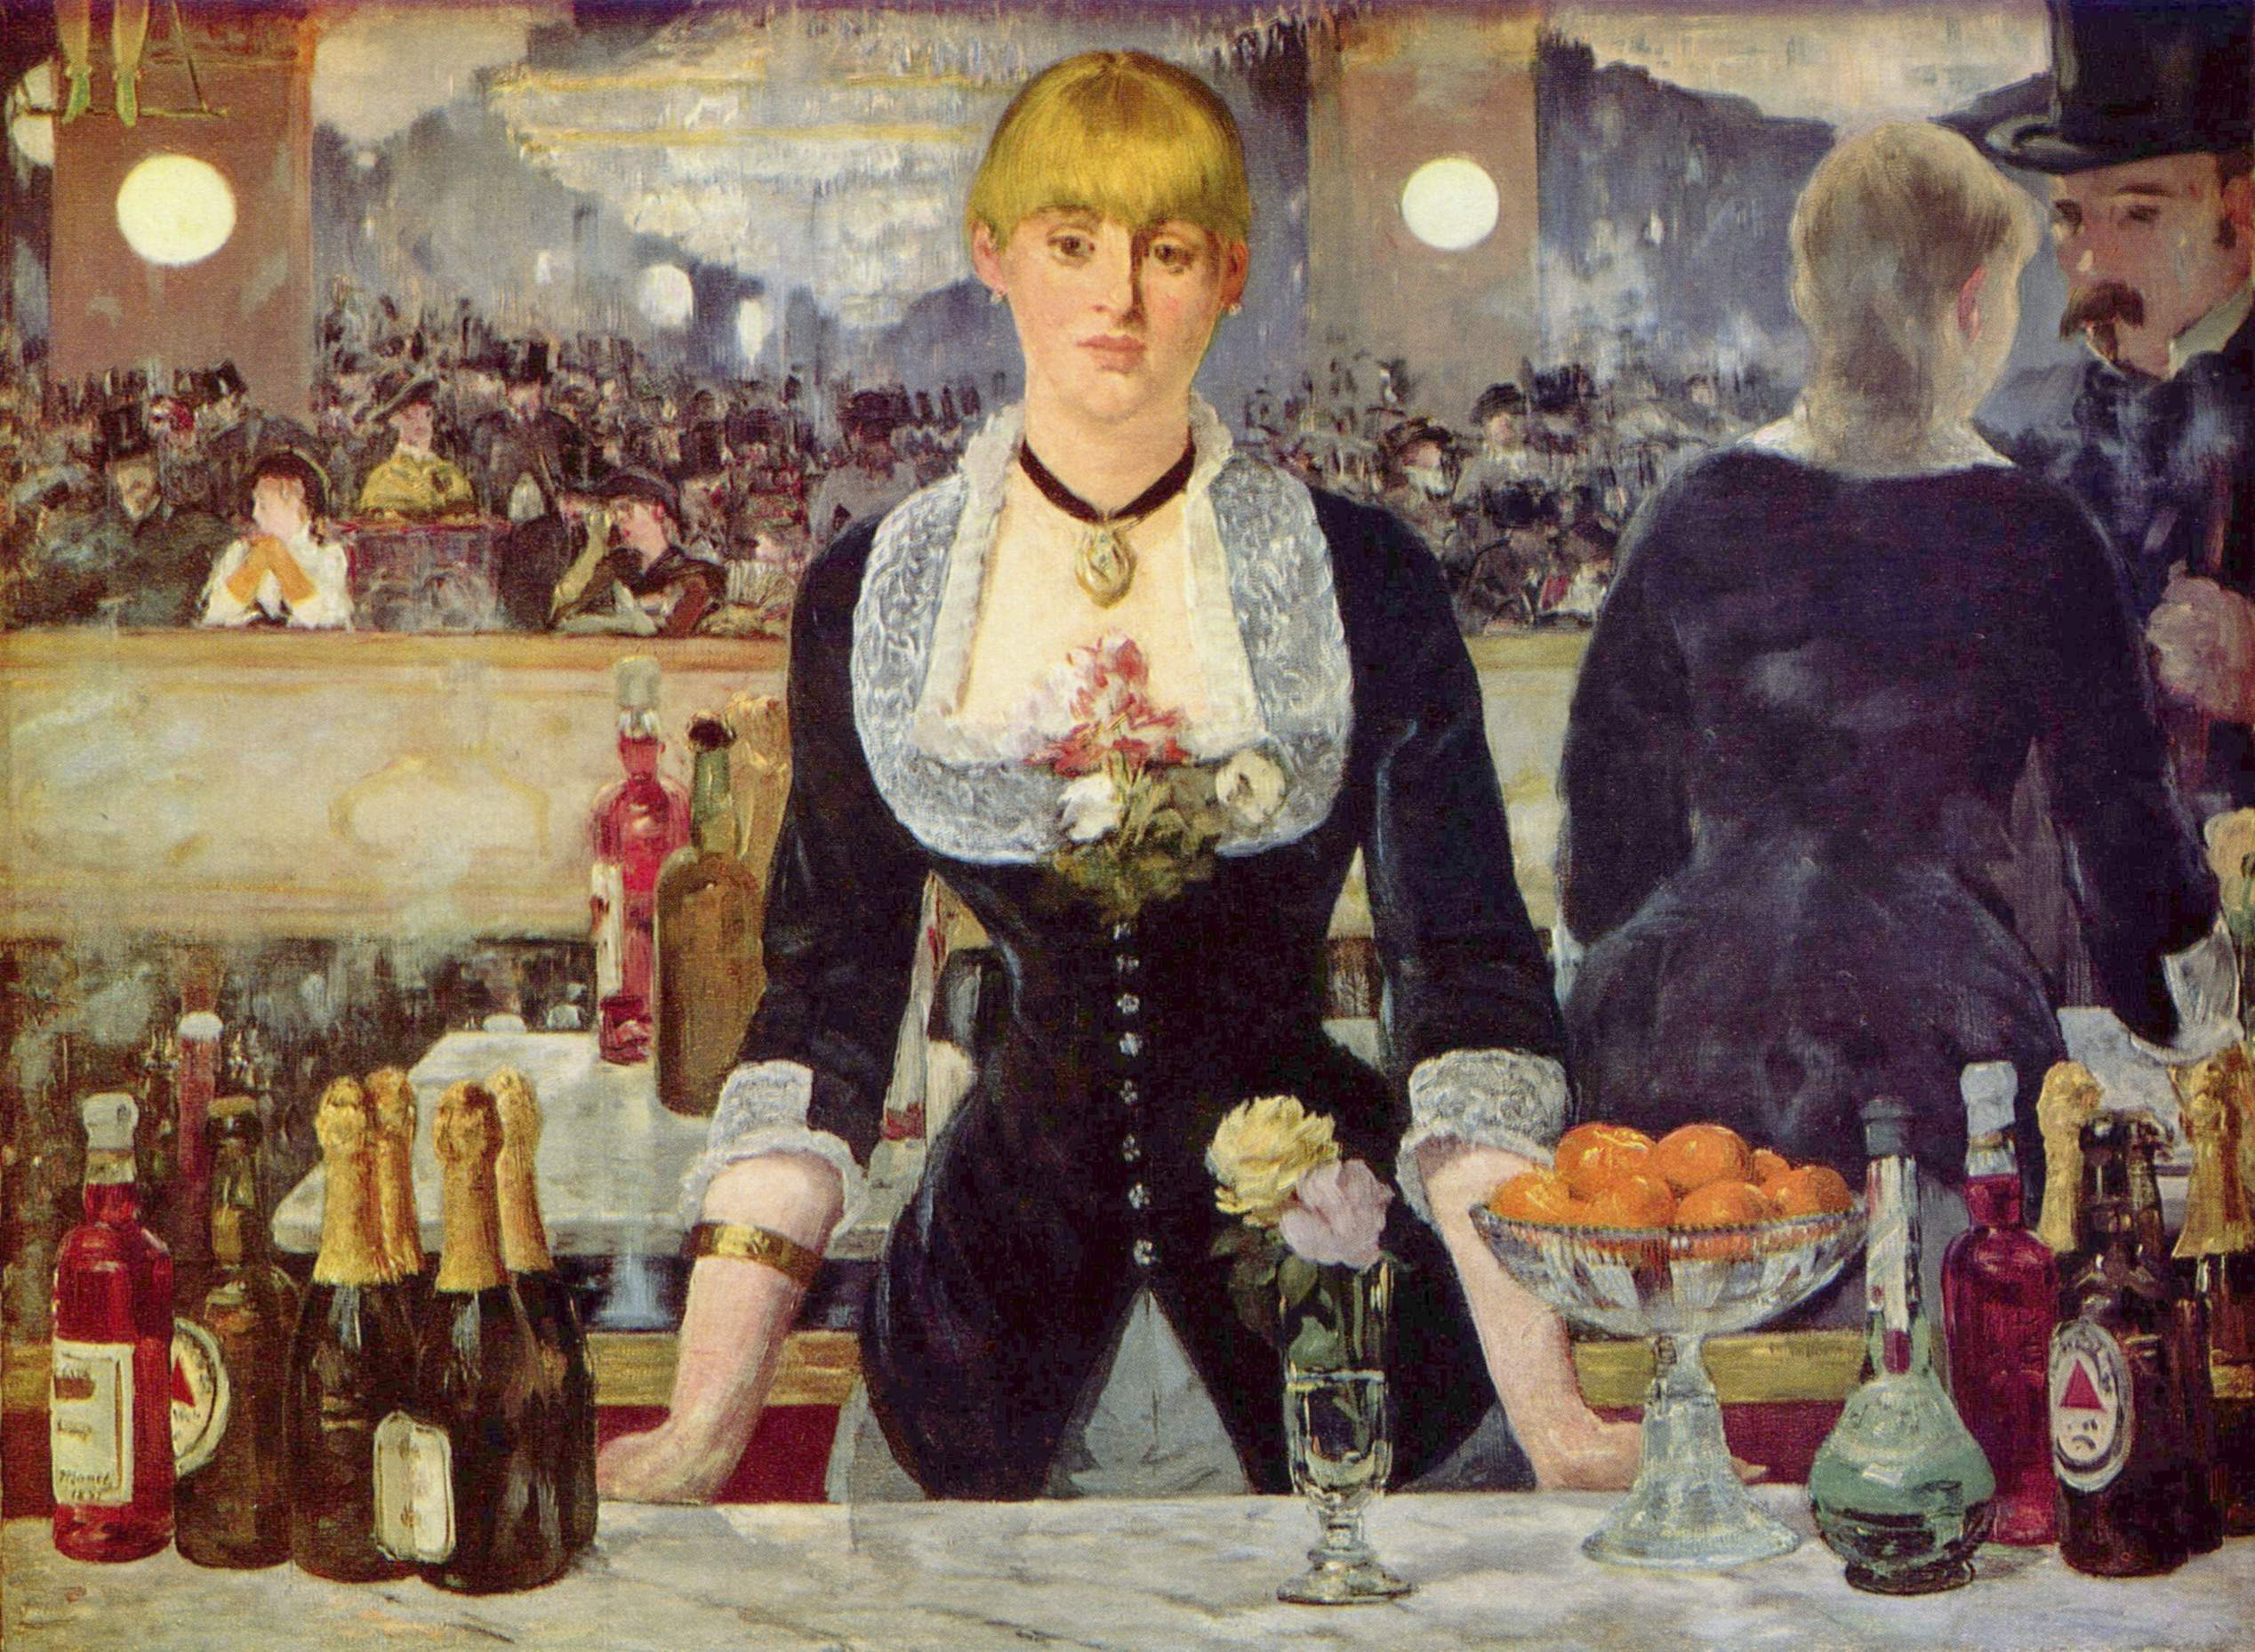
\includegraphics[width=1.25\textwidth]{./chapters/manet}\par
    \par\hfill\hfill{\tiny\bfseries Manet's  \textit{The Barmaid.}}\\
    \par
    \vspace*{\baselineskip}
    \par\hfill},
 title after={\hfill\hfill},
 title font-family=\sffamily,
 title font-color=\color{black!80},
 title font-weight=\bfseries,
 title font-size=\LARGE}}

\cxset{manet}
\chapter{EDOUARD MANET}
\buildptc
\section{dos columnas}
\begin{multicols}{3}
      \leftskip0pt
      \lettrine{I}{psum dolor} sit amet latixeus. \lipsum*[1-2]
      Latinicus porcupinus to fill the line.
\end{multicols}
\section{una columna}
\lipsum*[1-2]

%% CARDINAL

\cxset{manet}

\def\topimage#1{\cxset{title before={\hskip-2.3cm\includegraphics[width=1.25\textwidth]{./chapters/#1}\par
\vspace*{\baselineskip}\par}}}

\cxset{manet}
\topimage{piramide}

\chapter{ALAN MacDONALD}
\buildptc
\section{tres columnas}
\begin{multicols}{3}
      \leftskip0pt
      \lettrine{I}{psum dolor} sit amet latixeus. \lipsum*[1-2]
      Latinicus porcupinus to fill the line.
\end{multicols}
\clearpage
\section{una columna}
This particular code, uses the predefined style \textit{manet}. The only difference we have now defined a helper macro to make it easier for such images to be inserted for similar style chapter openings.

\medskip

\begin{lstlisting}
\def\topimage#1{\cxset{title before={\hskip-2.3cm\includegraphics[width=1.25\textwidth]{./chapters/#1}\par
\vspace*{\baselineskip}\par}}}
\end{lstlisting}
\section{una mas}
If a full book is to be designed using chapter openings in this fashion more keys and styles could be defined to make it even more easy to enter.

The full code to have the chapter typeset is shown below:
\medskip

\begin{lstlisting}
\cxset{manet}
\topimage{Alan-MacDonald-Cardinal-Spin-01}

\chapter{ALAN MacDONALD}
\begin{multicols}{3}
      \leftskip0pt
      \lettrine{I}{psum dolor} sit amet latixeus. \lipsum*[1-2]
      Latinicus porcupinus to fill the line.
\end{multicols}
\end{lstlisting}
All major components are saved in boxes. then based on booleans or templets are inserted in right location. Similar to objects.

\clearpage
%% GENETICS
\cxset{
 name={CHAPTER CONCEPT},
 numbering=none,
 number font-size=,
 number font-family=,
 number font-weight=,
 number color=white,
 chapter color={black},
 chapter font-family=\sffamily,
 chapter font-size=\large,
 chapter font-weight=\bfseries,
 title font-family=\sffamily,
 title font-color=teal,
 rule off,
}


\begin{specialchapter}[
     image=piramide,%genetics-dogs,
     %image caption={\minitoc}
     ]%
{Extensions\\ of Mendelian\\ Genetics}
\begin{itemize}
\item While alleles are transmitted from parent to   offspring
according to Mendelian principles, they often do not
display the clear-cut dominant/recessive relationship
observed by Mendel.
\item In many cases, in a departure from Mendelian genetics,
two or more genes are known to influence the phenotype
of a single characteristic.
\item Still another exception to Mendelian inheritance occurs
when genes are located on the X chromosome, because one
of the sexes receives only one copy of that chromosome,
eliminating the possibility of heterozygosity.
\item Phenotypes are often the combined result of genetics and
the environment within which genes are expressed.
\item The result of the various exceptions to Mendelian principles
is the occurrence of phenotypic ratios that differ from those
produced by standard monohybrid, dihybrid, and trihybrid
crosses.
  \end{itemize}
\end{specialchapter}
\cxset{name={},}
\ecap
%\chapter
\lipsum[1-2]
\chapter{Introduction}
%\buildptc
The aim of the package is to allow easy styling of chapter heads and extends these to include images and special effects, which are difficult to achieve using traditional methods. 

Abstracting the various designs is a non-trivial undertaking due to the hundreds of different possibilities.


\end{document}
